\documentclass[11pt,border=5pt]{standalone}
\usepackage{fontspec}
\setmainfont{cmunrm.otf}[BoldFont=cmunbx.otf,ItalicFont=cmunti.otf,BoldItalicFont=cmunbi.otf]
\usepackage{amsmath}
\usepackage{unicode-math}
\setmathfont{NewCMMath-Regular.otf}
\usepackage{tikz}
\usetikzlibrary{arrows.meta,patterns,angles,quotes}
\begin{document}
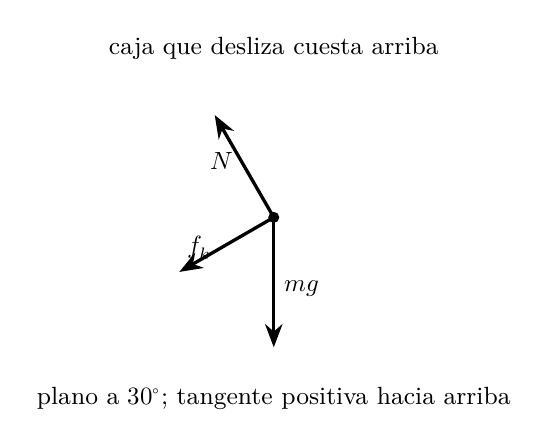
\begin{tikzpicture}[>=Stealth,font=\small,line cap=round,line join=round]
\fill (0,0) circle (2pt);
\draw[->,very thick] (0,0) -- (-0.75,1.3) node[pos=0.55,left] {$N$};
\draw[->,very thick] (0,0) -- (0,-1.65) node[pos=0.55,right] {$mg$};
\draw[->,very thick] (0,0) -- (-1.2,-0.693) node[pos=0.55,left] {$f_k$};
\node at (0,2.15) {caja que desliza cuesta arriba};
\node at (0,-2.3) {plano a $30^\circ$; tangente positiva hacia arriba};

\end{tikzpicture}
\end{document}
